\documentclass[10pt]{article}

\usepackage[a3paper, left=15mm,right=10mm, top=8mm, bottom=8mm, headheight=10pt]{geometry}
\usepackage{pgfpages}
\pgfpagesuselayout{resize to}[a4paper]

\usepackage[T1]{fontenc}
\usepackage[sfdefault,lining,scaled=.96]{FiraSans}
\usepackage[lining,scaled=.96]{FiraMono}
\usepackage{concmath}

\usepackage{amssymb}
\usepackage{tabularx,booktabs,multirow}

\usepackage{enumitem}
\setlist{nosep}

\usepackage{fancyvrb}

\usepackage{titlesec}
\titleformat{\section}{\large\bfseries\scshape}{\thesection}{1ex}{}
\titlespacing{\section}{0pt}{1ex}{0pt}

\usepackage{multicol}
\usepackage{tabto}
\usepackage{grid-system}

\usepackage{bytefield}
\usepackage{karnaugh-map,adjustbox}
\usepackage{tikz}
\usepackage[american]{circuitikz}
\ctikzset{
    logic ports=ieee,
    logic ports/scale=0.7,
}


\setlength\parindent{0pt}

\begin{document}

\thispagestyle{empty}

\textbf{\Huge MIPS Reference Sheet}

\vspace{1em}

\begin{minipage}[t]{0.68\linewidth}
    \centering
\hyphenation{Unsigned}
\renewcommand{\thefootnote}{\alph{footnote}}
\newcolumntype{O}{>{\centering\arraybackslash}c}
\newcolumntype{N}{>{\raggedright\arraybackslash\hangindent=4ex}p{16em}}
\newcolumntype{M}{>{\tt}l}
\newcolumntype{D}{>{\raggedright\arraybackslash\hangindent=4ex}X}

\begin{tabularx}{\textwidth}{NMcDcO}
    \toprule
    \multicolumn{3}{c}{\textsc{Name, Mnemonic, Format}} & \multicolumn{1}{c}{\textsc{Description}} &   & \textsc{Opcode/Funct}                                                                             \\
    \midrule
    Add                                                 & add                                      & R & R[rd] = R[rs] + R[rt]                                 & \footnotemark[1]                 & 0/0x20 \\
    Add Unsigned                                        & addu                                     & R & R[rd] = R[rs] + R[rt]                                 &                                  & 0/0x21 \\
    Add Imm.                                            & addi                                     & I & R[rt] = R[rs] + SignExtImm                            & \footnotemark[1]\footnotemark[2] & 0x08   \\
    Add Imm. Unsigned                                   & addiu                                    & I & R[rt] = R[rs] + SignExtImm                            & \footnotemark[2]                 & 0x09   \\
    Subtract                                            & sub                                      & R & R[rd] = R[rs] - R[rt]                                 &                                  & 0/0x22 \\
    Subtract Unsigned                                   & subu                                     & R & R[rd] = R[rs] - R[rt]                                 &                                  & 0/0x23 \\
    Shift Left Logical                                  & sll                                      & R & R[rd] = R[rt] <{}< shamt                              &                                  & 0/0x00 \\
    Shift Right Logical                                 & srl                                      & R & R[rd] = R[rt] >{}>{}> shamt                           &                                  & 0/0x02 \\
    \midrule
    And                                                 & and                                      & R & R[rd] = R[rs] \& R[rt]                                &                                  & 0/0x24 \\
    And Imm.                                            & andi                                     & I & R[rt] = R[rs] \& ZeroExtImm                           & \footnotemark[3]                 & 0x0c   \\
    Or                                                  & or                                       & R & R[rd] = R[rs] | R[rt]                                 &                                  & 0/0x25 \\
    Or Imm.                                             & ori                                      & I & R[rt] = R[rs] | ZeroExtImm                            & \footnotemark[3]                 & 0x0d   \\
    Exclusive-Or                                        & xor                                      & R & R[rd] = R[rs] \textasciicircum{} R[rt]                &                                  & 0/0x26 \\
    Exclusive-Or Imm.                                   & xori                                     & I & R[rt] = R[rs] \textasciicircum{} ZeroExtImm           & \footnotemark[3]                 & 0x0e   \\
    Nor                                                 & nor                                      & R & R[rd] = ~ (R[rs] | R[rt])                             &                                  & 0/0x27 \\
    \midrule
    Set Less Than                                       & slt                                      & R & R[rd] = (R[rs] < R[rt]) ? 1 : 0                       &                                  & 0/0x2a \\
    Set Less Than Unsigned                              & sltu                                     & R & R[rd] = (R[rs] < R[rt]) ? 1 : 0                       & \footnotemark[6]                 & 0/0x2b \\
    Set Less Than Imm.                                  & slti                                     & I & R[rt] = (R[rs] < SignExtImm)? 1 : 0                   & \footnotemark[2]                 & 0x0a   \\
    Set Less Than Imm. Unsigned                         & sltiu                                    & I & R[rt] = (R[rs] < SignExtImm) ? 1 : 0                  & \footnotemark[2]\footnotemark[6] & 0x0b   \\
    \midrule
    Branch On Equal                                     & beq                                      & I & if(R[rs]==R[rt]) PC=PC+4+BranchAddr                   & \footnotemark[4]                 & 0x04   \\
    Branch On Not Equal                                 & bne                                      & I & if(R[rs]!=R[rt]) PC=PC+4+BranchAddr                   & \footnotemark[4]                 & 0x05   \\
    Jump                                                & j                                        & J & PC=JumpAddr                                           & \footnotemark[5]                 & 0x02   \\
    Jump And Link                                       & jal                                      & J & R[31]=PC+8; PC=JumpAddr                               & \footnotemark[5]\footnotemark[7] & 0x03   \\
    Jump Register                                       & jr                                       & R & PC=R[rs]                                              &                                  & 0/0x08 \\
    \midrule
    Load Byte Unsigned                                  & lbu                                      & I & R[rt]={24'b0,M[R[rs] +SignExtImm](7:0)}               & \footnotemark[2]                 & 0x24   \\
    Load Halfword Unsigned                              & lhu                                      & I & R[rt]={16'b0,M[R[rs]+SignExtImm](15:0)}               & \footnotemark[2]                 & 0x25   \\
    Load Linked                                         & ll                                       & I & R[rt] = M[R[rs]+SignExtImm]                           & \footnotemark[2]\footnotemark[7] & 0x30   \\
    Load Upper Imm.                                     & lui                                      & I & R[rt] = {imm, 16'b0}                                  &                                  & 0x0f   \\
    Load Word                                           & lw                                       & I & R[rt] = M[R[rs]+SignExtImm]                           & \footnotemark[2]                 & 0x23   \\
    Store Byte                                          & sb                                       & I & M[R[rs]+SignExtImm](7:0) = R[rt](7:0)                 & \footnotemark[2]                 & 0x28   \\
    Store Conditional                                   & sc                                       & I & M[R[rs]+SignExtImm] = R[rt]; R[rt] = (atomic) ? 1 : 0 & \footnotemark[2]                 & 0x38   \\
    Store Halfword                                      & sh                                       & I & M[R[rs]+SignExtImm](15:0) = R[rt](l5:0)               & \footnotemark[2]                 & 0x29   \\
    Store Word                                          & sw                                       & I & M[R[rs]+SignExtImm] = R[rt]                           & \footnotemark[2]                 & 0x2b   \\
    \bottomrule
\end{tabularx}

\begin{minipage}[t]{\linewidth-4em}
    \begin{multicols}{2}
        \footnotesize
        \footnotemark[1]{May cause overflow exception}    \\
        \footnotemark[2]{SignExtImm = \{16\{immediate[15]\}, immediate\}} \\
        \footnotemark[3]{ZeroExtImm = \{16\{1b'0\}, immediate\}}    \\
        \footnotemark[4]{BranchAddr = \{14\{immediate[15]\}, immediate, 2'b0\}} \\
        \footnotemark[5]{JumpAddr = \{PC+4[31:28], address, 2'b0\}}    \\
        \footnotemark[6]{Operands considered unsigned numbers (vs. 2's comp.)}    \\
        \footnotemark[7]{Atomic test \& set pair; R[rt] = 1 if pair atomic, 0 if not atomic}
    \end{multicols}
\end{minipage}


    % \section*{Register Name, Number, Use, Call Convention}

% \newcolumntype{U}{>{\raggedright\arraybackslash\hangindent=4ex}X}
% \begin{tabularx}{\textwidth}{llUc}
%     \toprule
%     \textsc{Name}  & \textsc{Number} & \multicolumn{1}{c}{\textsc{Use}}                      & \textsc{Preserved on Call?} \\
%     \midrule
%     \verb|$zero|   & 0               & The constant value 0                                  & N.A.                \\
%     \verb|$at|     & 1               & Assembler temporary                                   & No                  \\
%     \verb|$v0-$v1| & 2-3             & Values for function results and expression evaluation & No                  \\
%     \verb|$a0-$a3| & 4-7             & Arguments                                             & No                  \\
%     \verb|$t0-$t7| & 8-15            & Temporaries                                           & No                  \\
%     \verb|$s0-$s7| & 16-23           & Saved temporaries                                     & Yes                 \\
%     \verb|$t8-$t9| & 24-25           & Temporaries                                           & No                  \\
%     \verb|$k0-$k1| & 26-27           & Reserved for os kernel                                & No                  \\
%     \verb|$gp|     & 28              & Global pointer                                        & Yes                 \\
%     \verb|$sp|     & 29              & Stack pointer                                         & Yes                 \\
%     \verb|$fp|     & 30              & Frame pointer                                         & Yes                 \\
%     \verb|$ra|     & 31              & Return address                                        & Yes                 \\
%     \bottomrule
% \end{tabularx}


\section*{Register Name, Number, Use}

\newcolumntype{U}{>{\raggedright\arraybackslash\hangindent=4ex}X}
\begin{tabularx}{\textwidth}{llU}
    \toprule
    \textsc{Name}  & \textsc{Num} & \multicolumn{1}{c}{\textsc{Use}}                    \\
    \midrule
    \verb|$zero|   & 0               & The constant value 0                                           \\
    \verb|$at|     & 1               & Assembler temporary                                            \\
    \verb|$v0-$v1| & 2-3             & Values for function results and expression evaluation          \\
    \verb|$a0-$a3| & 4-7             & Arguments                                                      \\
    \verb|$t0-$t7| & 8-15            & Temporaries                                                    \\
    \verb|$s0-$s7| & 16-23           & Saved temporaries                                              \\
    \verb|$t8-$t9| & 24-25           & Temporaries                                                    \\
    \verb|$k0-$k1| & 26-27           & Reserved for os kernel                                         \\
    \verb|$gp|     & 28              & Global pointer                                                 \\
    \verb|$sp|     & 29              & Stack pointer                                                  \\
    \verb|$fp|     & 30              & Frame pointer                                                  \\
    \verb|$ra|     & 31              & Return address                                                 \\
    \bottomrule
\end{tabularx}


    \begin{minipage}[t]{0.71\linewidth}
        % chktex-file 44
\section*{Truth Tables}

\begin{Row}
	\begin{Cell}{1}
		\textbf{AND}\vspace{0.5ex}

		\centering
		\begin{circuitikz}[]
			\draw (0,0) 	node[and port](G){};
			\draw (G.in 1) 	node[anchor=east]{$a$};
			\draw (G.in 2) 	node[anchor=east]{$b$};
			\draw (G.out) 	node[anchor=west]{$a \cdot b$};
		\end{circuitikz}
	\end{Cell}
	\begin{Cell}{1}
		\textbf{OR}\vspace{0.5ex}

		\centering
		\begin{circuitikz}[]
			\draw (0,0) 	node[or port](G){};
			\draw (G.in 1) 	node[anchor=east]{$a$};
			\draw (G.in 2) 	node[anchor=east]{$b$};
			\draw (G.out) 	node[anchor=west]{$a + b$};
		\end{circuitikz}
	\end{Cell}
	\begin{Cell}{1}
		\textbf{XOR}\vspace{0.5ex}

		\centering
		\begin{circuitikz}[]
			\draw (0,0) 	node[xor port](G){};
			\draw (G.in 1) 	node[anchor=east]{$a$};
			\draw (G.in 2) 	node[anchor=east]{$b$};
			\draw (G.out) 	node[anchor=west]{$a \oplus b$};
		\end{circuitikz}
	\end{Cell}
	\begin{Cell}{1}
		\textbf{NOT}\vspace{0.5ex}

		\centering
		\begin{circuitikz}[]
			\draw (0,0) 	node[not port](G){};
			\draw (G.in) 	node[anchor=east]{$a$};
			\draw (G.out) 	node[anchor=west]{$\overline{a}$};
		\end{circuitikz}
	\end{Cell}
\end{Row}

\vspace{1ex}

\begin{Row}
	\begin{Cell}{1}
		\centering
		\begin{tabular}{cc|c}
			\toprule
			$a$ & $b$ & $a\cdot b$ \\
			\midrule
			$0$ & $0$ & $0$        \\
			$0$ & $1$ & $0$        \\
			$1$ & $0$ & $0$        \\
			$1$ & $1$ & $1$        \\
			\bottomrule
		\end{tabular}
	\end{Cell}
	\begin{Cell}{1}
		\centering
		\begin{tabular}{cc|c}
			\toprule
			$a$ & $b$ & $a+b$ \\
			\midrule
			$0$ & $0$ & $0$   \\
			$0$ & $1$ & $1$   \\
			$1$ & $0$ & $1$   \\
			$1$ & $1$ & $1$   \\
			\bottomrule
		\end{tabular}
	\end{Cell}
	\begin{Cell}{1}
		\centering
		\begin{tabular}{cc|c}
			\toprule
			$a$ & $b$ & $a \oplus b$ \\
			\midrule
			$0$ & $0$ & $0$          \\
			$0$ & $1$ & $1$          \\
			$1$ & $0$ & $1$          \\
			$1$ & $1$ & $0$          \\
			\bottomrule
		\end{tabular}
	\end{Cell}
	\begin{Cell}{1}
		\centering
		\begin{tabular}{c|c}
			\toprule
			$a$ & $\overline{a}$ \\
			\midrule
			$0$ & $1$            \\
			$1$ & $0$            \\
			\bottomrule
		\end{tabular}
	\end{Cell}
\end{Row}

\vspace{1em}

\begin{Row}
	\begin{Cell}{1}
		\textbf{NAND}\vspace{0.5ex}

		\centering
		\begin{circuitikz}[]
			\draw (0,0) 	node[nand port](G){};
			\draw (G.in 1) 	node[anchor=east]{$a$};
			\draw (G.in 2) 	node[anchor=east]{$b$};
			\draw (G.out) 	node[anchor=west]{$\overline{a \cdot b}$};
		\end{circuitikz}
	\end{Cell}
	\begin{Cell}{1}
		\textbf{NOR}\vspace{0.5ex}

		\centering
		\begin{circuitikz}[]
			\draw (0,0) 	node[nor port](G){};
			\draw (G.in 1) 	node[anchor=east]{$a$};
			\draw (G.in 2) 	node[anchor=east]{$b$};
			\draw (G.out) 	node[anchor=west]{$\overline{a + b}$};
		\end{circuitikz}
	\end{Cell}
	\begin{Cell}{1}
		\textbf{XNOR}\vspace{0.5ex}

		\centering
		\begin{circuitikz}[]
			\draw (0,0) 	node[xnor port](G){};
			\draw (G.in 1) 	node[anchor=east]{$a$};
			\draw (G.in 2) 	node[anchor=east]{$b$};
			\draw (G.out) 	node[anchor=west]{$\overline{a \oplus b}$};
		\end{circuitikz}
	\end{Cell}
	\begin{Cell}{1}
		\phantom{x}
	\end{Cell}
\end{Row}

\vspace{1ex}

\begin{Row}
	\begin{Cell}{1}
		\centering
		\begin{tabular}{cc|c}
			\toprule
			$a$ & $b$ & $\overline{a\cdot b}$ \\
			\midrule
			$0$ & $0$ & $1$                   \\
			$0$ & $1$ & $1$                   \\
			$1$ & $0$ & $1$                   \\
			$1$ & $1$ & $0$                   \\
			\bottomrule
		\end{tabular}
	\end{Cell}
	\begin{Cell}{1}
		\centering
		\begin{tabular}{cc|c}
			\toprule
			$a$ & $b$ & $\overline{a+b}$ \\
			\midrule
			$0$ & $0$ & $1$              \\
			$0$ & $1$ & $0$              \\
			$1$ & $0$ & $0$              \\
			$1$ & $1$ & $0$              \\
			\bottomrule
		\end{tabular}
	\end{Cell}
	\begin{Cell}{1}
		\centering
		\begin{tabular}{cc|c}
			\toprule
			$a$ & $b$ & $\overline{a \oplus b}$ \\
			\midrule
			$0$ & $0$ & $1$                     \\
			$0$ & $1$ & $0$                     \\
			$1$ & $0$ & $0$                     \\
			$1$ & $1$ & $1$                     \\
			\bottomrule
		\end{tabular}
	\end{Cell}
	\begin{Cell}{1}
		\phantom{x}
	\end{Cell}
\end{Row}

    \end{minipage}
    \hfill
    \begin{minipage}[t]{0.28\linewidth}
        \begin{tabular*}{\linewidth}{@{\extracolsep{\fill}}cccc}
    \toprule
    Value        & Sign \& Mag & 1s Comp.    & 2s Comp.      \\
    \midrule
    +7         & {0111}    & {0111} & {0111} \\
    +6         & {0110}    & {0110} & {0110} \\
    +5         & {0101}    & {0101} & {0101} \\
    +4         & {0100}    & {0100} & {0100} \\
    +3         & {0011}    & {0011} & {0011} \\
    +2         & {0010}    & {0010} & {0010} \\
    +1         & {0001}    & {0001} & {0001} \\
    +0         & {0000}    & {0000} & {0000} \\
    \midrule
    -0         & {1000}    & {1111} & {-}    \\
    -1         & {1001}    & {1110} & {1111} \\
    -2         & {1010}    & {1101} & {1110} \\
    -3         & {1011}    & {1100} & {1101} \\
    -4         & {1100}    & {1011} & {1100} \\
    -5         & {1101}    & {1010} & {1011} \\
    -6         & {1110}    & {1001} & {1010} \\
    -7         & {1111}    & {1000} & {1001} \\
    -8         & {-}       & {-}    & {1000} \\
    \bottomrule
\end{tabular*}

    \end{minipage}
\end{minipage}
\hfill
\begin{minipage}[t]{0.3\linewidth}
    \section*{Basic Instruction Formats}
\vspace{1ex}
\begin{itemize}[leftmargin=1em]
    \setlength\itemsep{1em}
    \item[R]
        \begin{bytefield}[boxformatting=\centering\small,bitwidth=0.03125\linewidth,bitheight=1.5em]{32}
            \bitheader[endianness=big]{0,5,6,10,11,15,16,20,21,25,26,31} \\
            \bitbox{6}{opcode} &
            \bitbox{5}{rs} &
            \bitbox{5}{rt} &
            \bitbox{5}{rd} &
            \bitbox{5}{shamt} &
            \bitbox{6}{funct}
        \end{bytefield}
    \item[I]
        \begin{bytefield}[boxformatting=\centering\small,bitwidth=0.03125\linewidth,bitheight=1.5em]{32}
            \bitheader[endianness=big]{0,15,16,20,21,25,26,31} \\
            \bitbox{6}{opcode} &
            \bitbox{5}{rs} &
            \bitbox{5}{rt} &
            \bitbox{16}{immediate}
        \end{bytefield}
    \item[J]
        \begin{bytefield}[boxformatting=\centering\small,bitwidth=0.03125\linewidth,bitheight=1.5em]{32}
            \bitheader[endianness=big]{0,25,26,31} \\
            \bitbox{6}{opcode} &
            \bitbox{26}{address}
        \end{bytefield}
\end{itemize}


    \section*{IEEE 754 Floating Point Standard}
$$
    (-1)^S \times M \times 2^{E-B}
$$

Single Precision Format (Bias = 127) \vspace{1em}
\begin{center}
    \begin{bytefield}[boxformatting=\centering\small,bitwidth=0.03\linewidth,bitheight=1.5em]{32}
        \bitheader[endianness=big]{0,22,23,30,31} \\
        \bitbox{1}{S} &
        \bitbox{8}{Exponent} &
        \bitbox{23}{Mantissa}
    \end{bytefield}
\end{center}

Double Precision Format (Bias = 1023)
\begin{center}
    \begin{bytefield}[boxformatting=\centering\small,bitwidth=0.03\linewidth,bitheight=1.5em]{32}
        \bitheader[lsb=32,endianness=big]{32,51,52,62,63} \\
        \bitbox{1}{S} &
        \bitbox{11}{Exponent} &
        \bitbox{20}{Mantissa[51:32]} \\
        \bitheader[endianness=big]{0,31} \\
        \bitbox{32}{Mantissa[31:0]}
    \end{bytefield}
\end{center}


    \section*{Base Convention, ASCII Symbols}

\newcolumntype{C}{>{\ttfamily}c}
\newcolumntype{R}{>{\ttfamily}r}
\begin{tabular*}{\linewidth}{@{\extracolsep{\fill}}C|RRC|RRC}
    \toprule
    BIN    & DEC & HEX & ASCII & DEC & HEX & ASCII            \\
    \midrule
    000000 & 0   & 0   & NUL   & 64  & 40  & @                \\
    000001 & 1   & 1   & SOH   & 65  & 41  & A                \\
    000010 & 2   & 2   & STX   & 66  & 42  & B                \\
    000011 & 3   & 3   & ETX   & 67  & 43  & C                \\
    000100 & 4   & 4   & EOT   & 68  & 44  & D                \\
    000101 & 5   & 5   & ENQ   & 69  & 45  & E                \\
    000110 & 6   & 6   & ACK   & 70  & 46  & F                \\
    000111 & 7   & 7   & BEL   & 71  & 47  & G                \\
    001000 & 8   & 8   & BS    & 72  & 48  & H                \\
    001001 & 9   & 9   & HT    & 73  & 49  & I                \\
    001010 & 10  & a   & LF    & 74  & 4a  & J                \\
    001011 & 11  & b   & VT    & 75  & 4b  & K                \\
    001100 & 12  & c   & FF    & 76  & 4c  & L                \\
    001101 & 13  & d   & CR    & 77  & 4d  & M                \\
    001110 & 14  & e   & SO    & 78  & 4e  & N                \\
    001111 & 15  & f   & SI    & 79  & 4f  & O                \\
    010000 & 16  & 10  & DLE   & 80  & 50  & P                \\
    010001 & 17  & 11  & DC1   & 81  & 51  & Q                \\
    010010 & 18  & 12  & DC2   & 82  & 52  & R                \\
    010011 & 19  & 13  & DC3   & 83  & 53  & S                \\
    010100 & 20  & 14  & DC4   & 84  & 54  & T                \\
    010101 & 21  & 15  & NAK   & 85  & 55  & U                \\
    010110 & 22  & 16  & SYN   & 86  & 56  & V                \\
    010111 & 23  & 17  & ETB   & 87  & 57  & W                \\
    011000 & 24  & 18  & CAN   & 88  & 58  & X                \\
    011001 & 25  & 19  & EM    & 89  & 59  & Y                \\
    011010 & 26  & 1a  & SUB   & 90  & 5a  & Z                \\
    011011 & 27  & 1b  & ESC   & 91  & 5b  & [                \\
    011100 & 28  & 1c  & FS    & 92  & 5c  & \textbackslash   \\
    011101 & 29  & 1d  & GS    & 93  & 5d  & ]                \\
    011110 & 30  & 1e  & RS    & 94  & 5e  & \textasciicircum \\
    011111 & 31  & 1f  & US    & 95  & 5f  & \textunderscore  \\
    100000 & 32  & 20  & Space & 96  & 60  & `                \\
    100001 & 33  & 21  & !     & 97  & 61  & a                \\
    100010 & 34  & 22  & "     & 98  & 62  & b                \\
    100011 & 35  & 23  & \#    & 99  & 63  & c                \\
    100100 & 36  & 24  & \$    & 100 & 64  & d                \\
    100101 & 37  & 25  & \%    & 101 & 65  & e                \\
    100110 & 38  & 26  & \&    & 102 & 66  & f                \\
    100111 & 39  & 27  & '     & 103 & 67  & g                \\
    101000 & 40  & 28  & (     & 104 & 68  & h                \\
    101001 & 41  & 29  & )     & 105 & 69  & i                \\
    101010 & 42  & 2a  & *     & 106 & 6a  & j                \\
    101011 & 43  & 2b  & +     & 107 & 6b  & k                \\
    101100 & 44  & 2c  & ,     & 108 & 6c  & l                \\
    101101 & 45  & 2d  & -     & 109 & 6d  & m                \\
    101110 & 46  & 2e  & .     & 110 & 6e  & n                \\
    101111 & 47  & 2f  & /     & 111 & 6f  & o                \\
    110000 & 48  & 30  & 0     & 112 & 70  & p                \\
    110001 & 49  & 31  & 1     & 113 & 71  & q                \\
    110010 & 50  & 32  & 2     & 114 & 72  & r                \\
    110011 & 51  & 33  & 3     & 115 & 73  & s                \\
    110100 & 52  & 34  & 4     & 116 & 74  & t                \\
    110101 & 53  & 35  & 5     & 117 & 75  & u                \\
    110110 & 54  & 36  & 6     & 118 & 76  & v                \\
    110111 & 55  & 37  & 7     & 119 & 77  & w                \\
    111000 & 56  & 38  & 8     & 120 & 78  & x                \\
    111001 & 57  & 39  & 9     & 121 & 79  & y                \\
    111010 & 58  & 3a  & :     & 122 & 7a  & z                \\
    111011 & 59  & 3b  & ;     & 123 & 7b  & \{               \\
    111100 & 60  & 3c  & <     & 124 & 7c  & |                \\
    111101 & 61  & 3d  & =     & 125 & 7d  & \}               \\
    111110 & 62  & 3e  & >     & 126 & 7e  & \textasciitilde  \\
    111111 & 63  & 3f  & ?     & 127 & 7f  & DEL              \\
    \bottomrule
\end{tabular*}

\end{minipage}

\vfill

\clearpage


\begin{minipage}[t]{0.64\linewidth}
    \section*{MIPS Data Path}
    \centering
    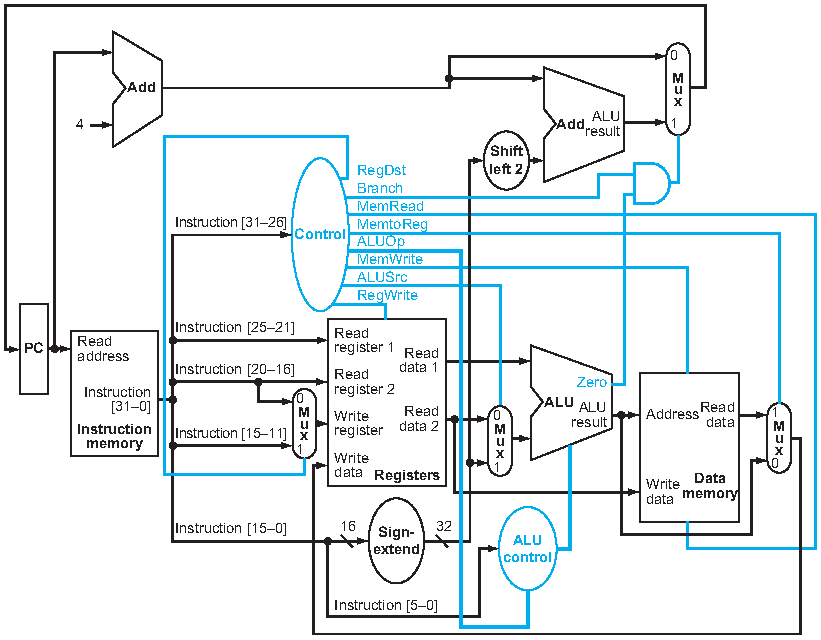
\includegraphics[width=\linewidth]{content/fig417.pdf}
\end{minipage}
\begin{minipage}[t]{0.35\linewidth}
    \section*{1-bit ALU}
    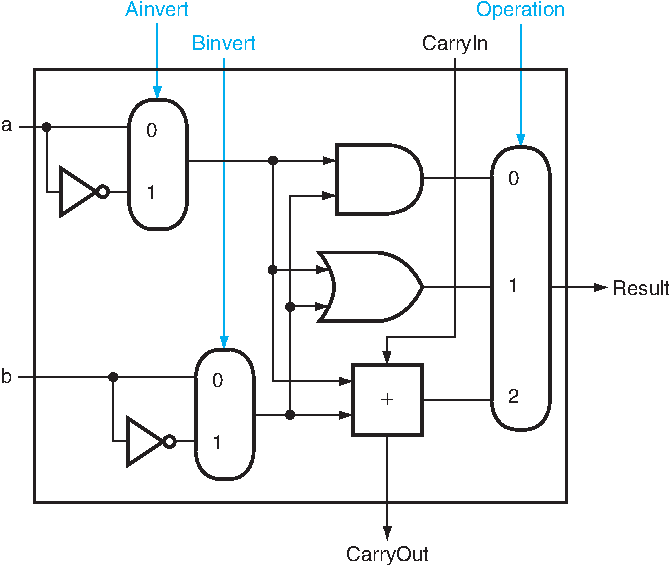
\includegraphics[width=\linewidth]{content/alu.pdf}
    \begin{center}
        \begin{tabular}[t]{c|ccc|c}
            \toprule
            ALUControl & Ainvert & Binvert & Operation & Action \\
            \midrule
            {\tt 0000} & 0       & 0       & 00        & AND    \\
            {\tt 0001} & 0       & 0       & 01        & OR     \\
            {\tt 0010} & 0       & 0       & 10        & ADD    \\
            {\tt 0110} & 0       & 1       & 10        & SUB    \\
            {\tt 0111} & 0       & 1       & 11        & SLT    \\
            {\tt 1100} & 1       & 1       & 00        & NOR    \\
            \bottomrule
        \end{tabular}
    \end{center}
\end{minipage}

\begin{minipage}[t]{\linewidth}
    \section*{MIPS Control Path}

    \begin{minipage}[t]{0.32\textwidth}
        \begin{tabular}[t]{ccccc}
    \toprule
             & R-type      & LW          & SW          & BEQ         \\
    \midrule
    RegDst   & \texttt{1}  & \texttt{0}  & \texttt{X}  & \texttt{X}  \\
    ALUSrc   & \texttt{0}  & \texttt{1}  & \texttt{1}  & \texttt{0}  \\
    MemToReg & \texttt{0}  & \texttt{1}  & \texttt{X}  & \texttt{X}  \\
    RegWrite & \texttt{1}  & \texttt{1}  & \texttt{0}  & \texttt{0}  \\
    MemRead  & \texttt{0}  & \texttt{1}  & \texttt{0}  & \texttt{0}  \\
    MemWrite & \texttt{0}  & \texttt{0}  & \texttt{1}  & \texttt{0}  \\
    Branch   & \texttt{0}  & \texttt{0}  & \texttt{0}  & \texttt{1}  \\
    ALUop    & \texttt{10} & \texttt{00} & \texttt{00} & \texttt{01} \\
    \bottomrule
\end{tabular}

    \end{minipage}
    \begin{minipage}[t]{0.64\textwidth}
        % \begin{tabular}{clcc}
%     \toprule
%     Operation & Opcode/Funct                & ALU Action & ALUOp/ALUCtrl             \\
%     \midrule
%     LW        & \texttt{0x23}               & add        & \texttt{00}/\texttt{0010} \\
%     SW        & \texttt{0x2b}               & add        & \texttt{00}/\texttt{0010} \\
%     BEQ       & \texttt{0x04}               & sub        & \texttt{01}/\texttt{0110} \\
%     ADD       & \texttt{0x00}/\texttt{0x20} & add        & \texttt{10}/\texttt{0010} \\
%     SUB       & \texttt{0x00}/\texttt{0x22} & sub        & \texttt{10}/\texttt{0110} \\
%     AND       & \texttt{0x00}/\texttt{0x24} & and        & \texttt{10}/\texttt{0000} \\
%     OR        & \texttt{0x00}/\texttt{0x25} & or         & \texttt{10}/\texttt{0001} \\
%     SLT       & \texttt{0x00}/\texttt{0x2a} & slt        & \texttt{10}/\texttt{0111} \\
%     \bottomrule
% \end{tabular}
\begin{tabular}[t]{cccccc}
    \toprule
    Opcode & ALUOp       & Operation        & Funct           & ALU action       & ALU control   \\
    \midrule
    LW     & {00} & load word        & {xxxxxx} & add              & {0010} \\
    SW     & {00} & store word       & {xxxxxx} & add              & {0010} \\
    BEQ    & {01} & branch equal     & {xxxxxx} & subtract         & {0110} \\
    R-type & {10} & add              & {100000} & add              & {0010} \\
    R-type & {10} & subtract         & {100010} & subtract         & {0110} \\
    R-type & {10} & AND              & {100100} & AND              & {0000} \\
    R-type & {10} & OR               & {100101} & OR               & {0001} \\
    R-type & {10} & set-on-less-than & {101010} & set-on-less-than & {0111} \\
    \bottomrule
\end{tabular}

    \end{minipage}
\end{minipage}

\vspace{1ex}

\begin{minipage}[t]{0.24\linewidth}
    \section*{K-Map}
\centering
\begin{karnaugh-map}(label=corner)[4][4][1][$D$][$C$][$B$][$A$]
\manualterms{$m_0$, $m_{1}$, $m_{2}$, $m_{3}$, $m_{4}$, $m_{5}$, $m_{6}$, $m_{7}$, $m_{8}$, $m_{9}$, $m_{10}$, $m_{11}$, $m_{12}$, $m_{13}$, $m_{14}$, $m_{15}$}
\end{karnaugh-map}

\end{minipage}
\begin{minipage}[t]{0.72\linewidth}
    \section*{Laws of Boolean Algebra}
\begin{tabular}{lll}
    \toprule
    \textbf{Name}           & \textbf{AND}                                                  & \textbf{OR}                                  \\
    \midrule
    Identity Laws           & $x \cdot 1 = x$                                               & $x + 0 = x$                                  \\
    Inverse/Complement Laws & $x \cdot x' = 0$                                              & $x + x' = 1$                                 \\
    Commutative Laws        & $x \cdot y = y \cdot x$                                       & $x + y = y + x$                              \\
    Associative Laws        & $x \cdot (y \cdot z) = (x \cdot y) \cdot z$                   & $x + (y + z) = (x + y) + z$                  \\
    Distributive Laws       & $x \cdot (y + z) = x \cdot y + x \cdot z$                     & $x + y \cdot z = (x + y) \cdot (x + z)$      \\
    \midrule
    Idempotency             & $x \cdot x = x$                                               & $x + x = x$                                  \\
    Zero/One Element        & $x \cdot 0 = 0$                                               & $x + 1 = 1$                                  \\
    Involution              & $(x')' = x$                                                   &                                              \\
    Absorption 1            & $x + x \cdot y = x$                                           & $x \cdot (x + y) = x$                        \\
    Absorption 2            & $x + x' \cdot y = x + y$                                      & $x \cdot (x' + y) = x \cdot y$               \\
    DeMorgan's Law          & $(x \cdot y)' = x' + y'$                                      & $(x + y)' = x' \cdot y'$                     \\
    Consensus               & $x \cdot y + x' \cdot z + y \cdot z = x \cdot y + x' \cdot z$ & $x + y \cdot z + x' \cdot z = x + y \cdot z$ \\
    \bottomrule
\end{tabular}

\end{minipage}

\end{document}
